% !TEX encoding = UTF-8 Unicode
\documentclass[12pt,a4paper]{report}
 
\usepackage[brazil]{babel}
\usepackage[utf8]{inputenc}
\usepackage[T1]{fontenc}
\usepackage{graphicx, subfigure, float}
\usepackage{epstopdf}
\usepackage{indentfirst}
\usepackage{fancyhdr}

\graphicspath{ {../images/} }

\epstopdfsetup{outdir=./}
\epstopdfsetup{suffix=}

\pagestyle{fancy}

\fancyhead[RO,RE]{
\includegraphics{unb.eps}}
\fancyhead[LO,LE]{Departamento de Ciência da Computação\\
116441 --- Engenharia de Software}

\fancypagestyle{plain}{
\fancyhead[RO,RE]{
\includegraphics{unb.eps}}
\fancyhead[LO,LE]{Departamento de Ciência da Computação\\
116441 --- Engenharia de Software}}

\title{Diagramas de Sequência do Sistema de Gestão Eletrônica de Documentos da Defensoria Pública do Distrito Federal - SGED/DPDF}
\author{Pedro Salum\\
	09/0139232\\
	pedro@loopec.com.br
	\and
	Daniel Sandoval\\
	09/0109899\\
	daniel@loopec.com.br}
	
\begin{document}
\maketitle
\tableofcontents

\chapter{Diagramas de Sequência}

\section{Login}
\begin{figure}[H]
\centering
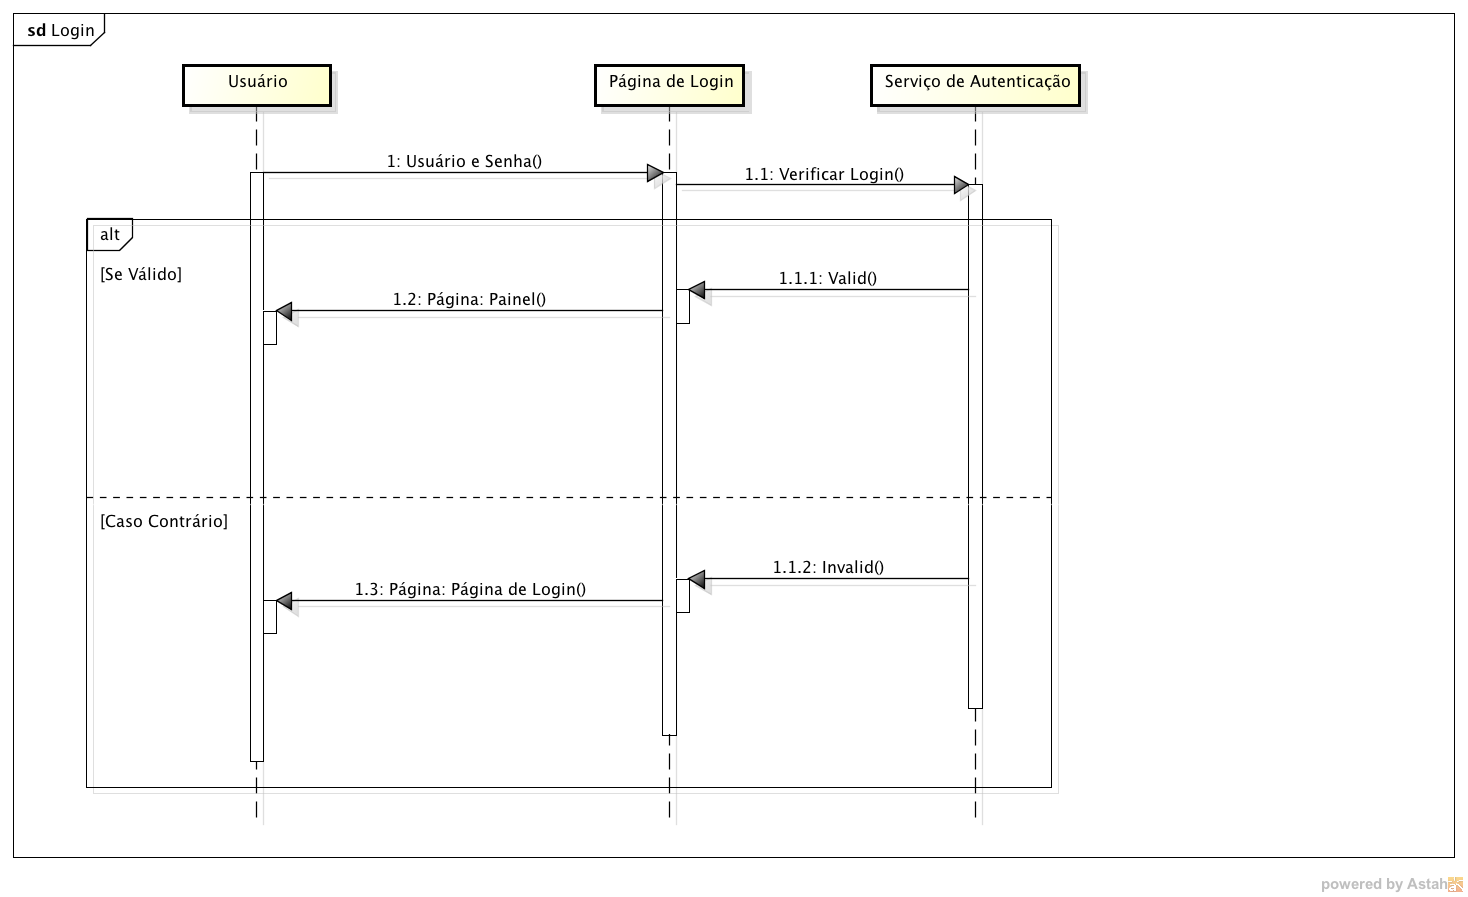
\includegraphics[width=\textwidth]{login.png}
\caption{Login}
\label{fig:login}
\end{figure}

\section{Entrada de Processos}
\begin{figure}[H]
\centering
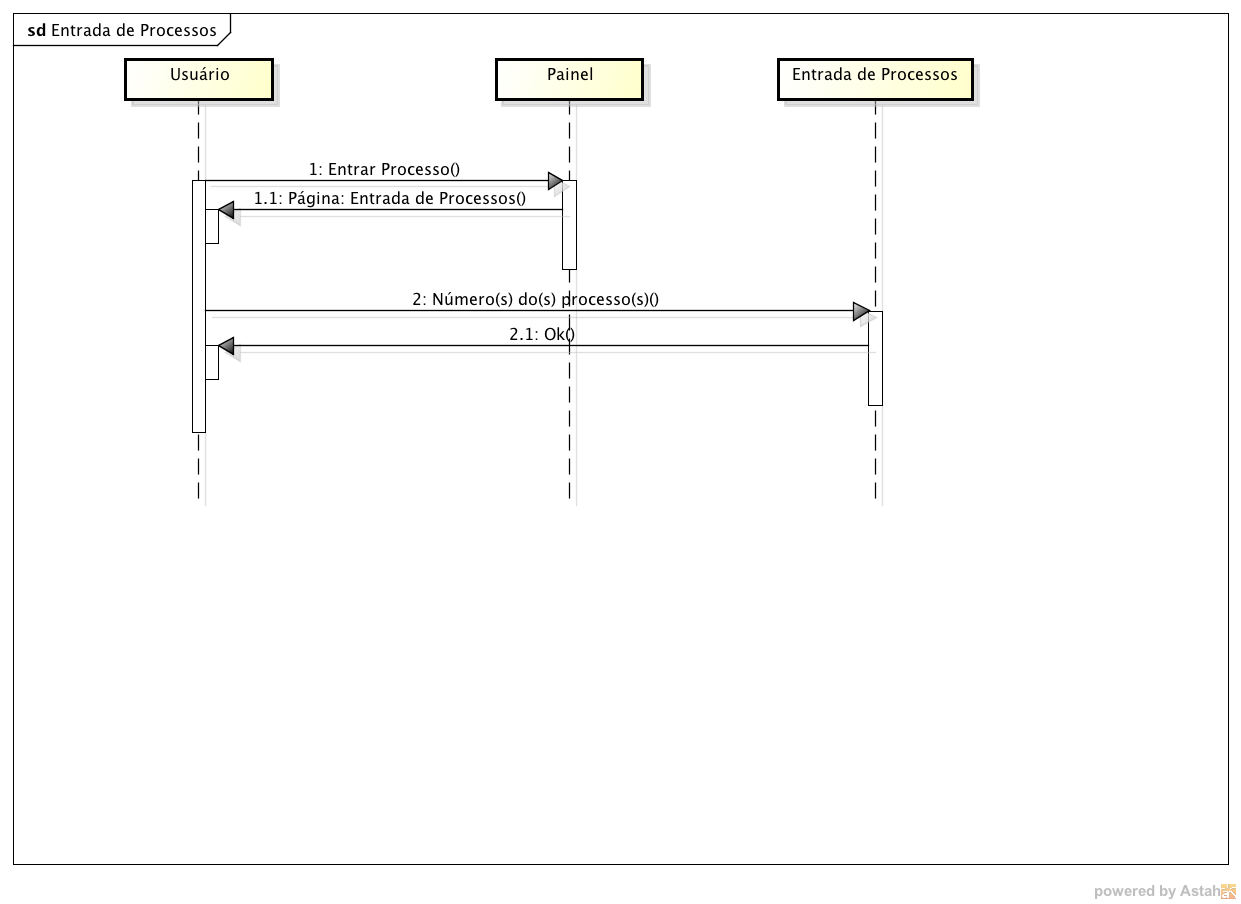
\includegraphics[width=\textwidth]{entrada-de-processos.png}
\caption{Entrada de Processos}
\label{fig:entrada}
\end{figure}

\section{Movimentação de Processos}
\begin{figure}[H]
\centering
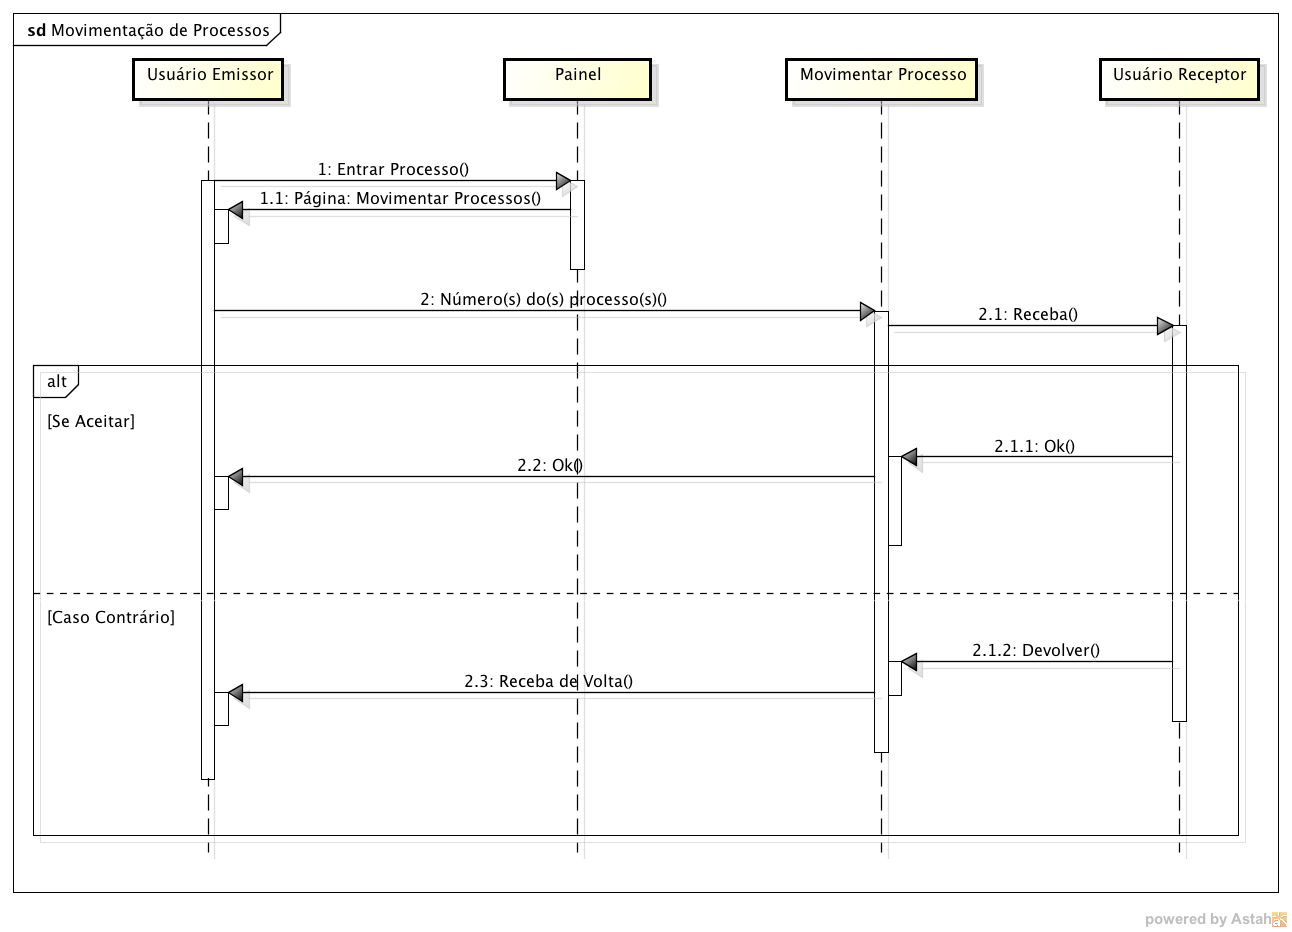
\includegraphics[width=\textwidth]{movimentacao-de-processos.png}
\caption{Movimentação de Processos}
\label{fig:movimentacao}
\end{figure}

\section{Escrever Peça}
\begin{figure}[H]
\centering
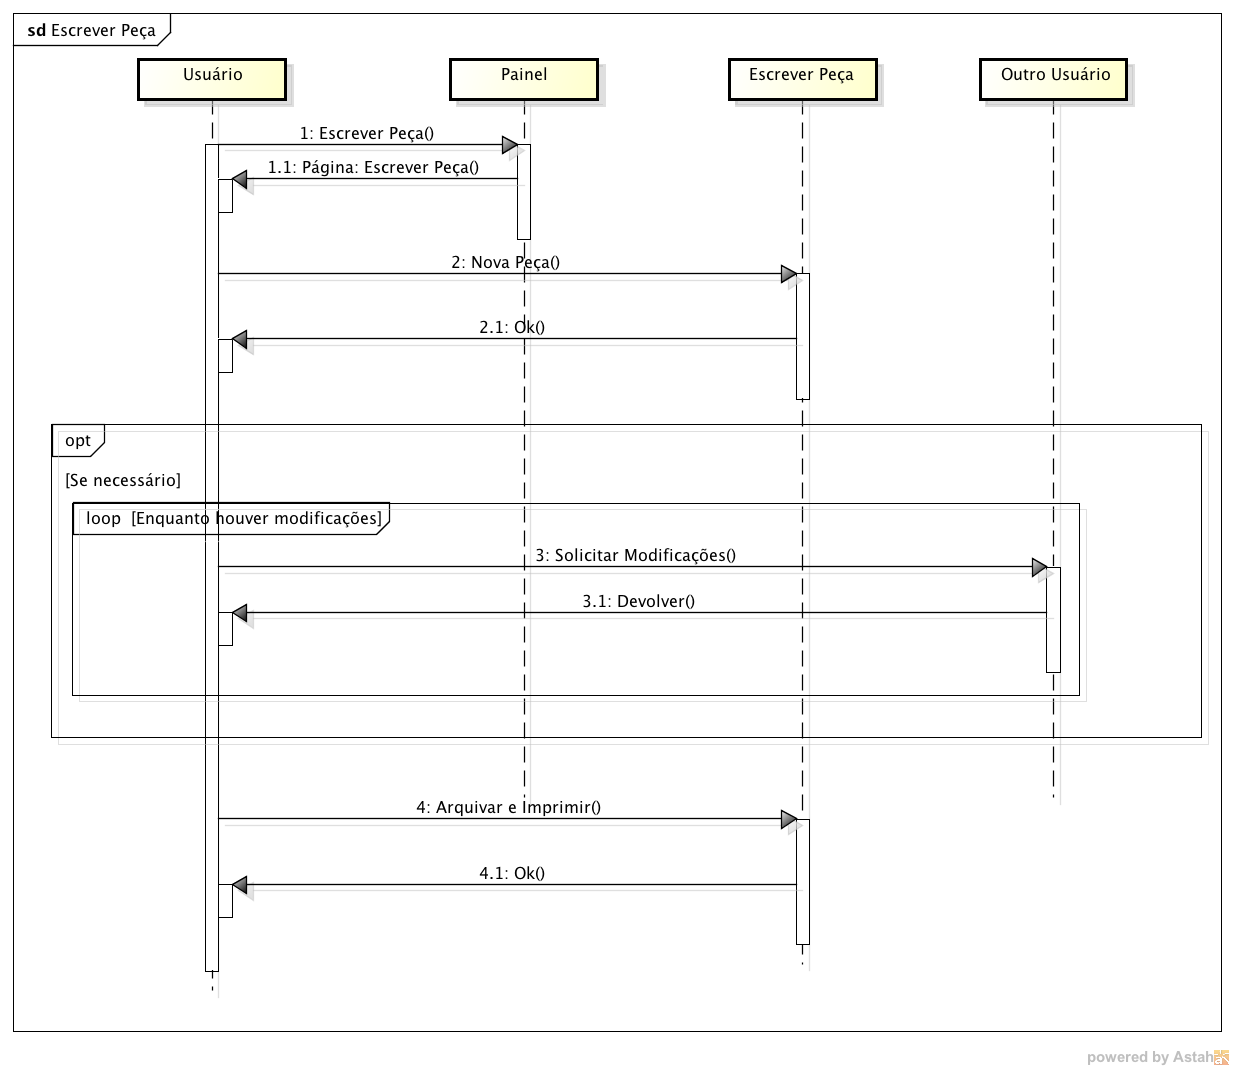
\includegraphics[width=\textwidth]{escrever-peca.png}
\caption{Escrever Peça}
\label{fig:escrever}
\end{figure}

\section{Inserir Documento Digitalizado}
\begin{figure}[H]
\centering
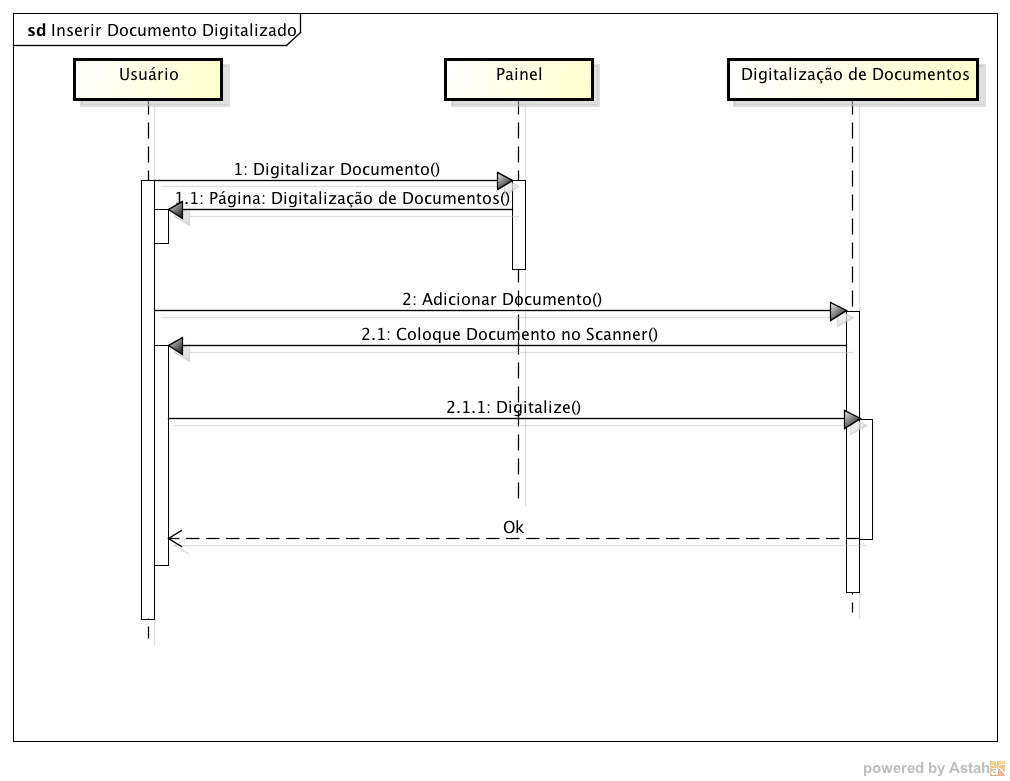
\includegraphics[width=\textwidth]{inserir-documento-digitalizado.png}
\caption{Inserir Documento Digitalizado}
\label{fig:digitalizar}
\end{figure}

\end{document}
